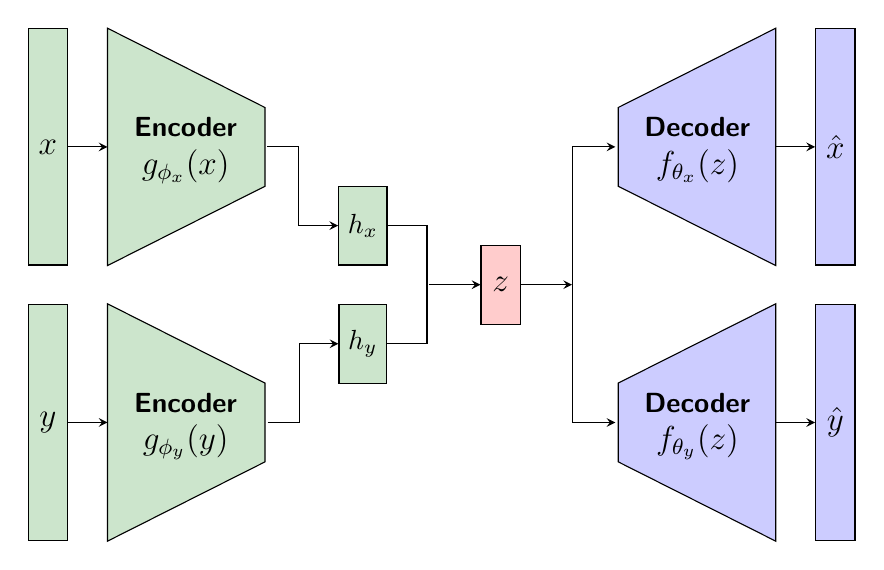
\begin{tikzpicture}
	
	\node[fill=Green!20, minimum width=0.5cm, minimum height=3.0cm, draw] (y) at (0,0) {\large $\boldsymbol y$};
	
	\node[fill=Green!20, minimum width=0.5cm, minimum height=3.0cm, draw] (x) at (0,3.5) {\large $\boldsymbol x$};
	
	\draw[fill=Green!20] ([xshift=0.5cm]x.north east) -- ([xshift=2.5cm,yshift=0.5cm]x.east) -- ([xshift=2.5cm,yshift=-0.5cm]x.east) -- ([xshift=0.5cm]x.south east) -- cycle; 
	\node at (1.75,3.75) {{\sf \textbf{Encoder}}};
	\node at (1.75,3.25) {\large $g_{\boldsymbol{\phi_x}}(\boldsymbol{x})$};
	
	
	\draw[fill=Green!20] ([xshift=0.5cm]y.north east) -- ([xshift=2.5cm,yshift=0.5cm]y.east) -- ([xshift=2.5cm,yshift=-0.5cm]y.east) -- ([xshift=0.5cm]y.south east) -- cycle; 
	\node at (1.75,0.25) {{\sf \textbf{Encoder}}};
	\node at (1.75,-0.25) {\large $g_{\boldsymbol{\phi_y}}(\boldsymbol{y})$};
	
	
	\node[fill=Green!20, minimum width=0.6cm, minimum height=1.0cm, draw] (hx) at (4.0cm,2.5cm) { $\boldsymbol{h_x}$};
	\node[fill=Green!20, minimum width=0.6cm, minimum height=1.0cm, draw] (hy) at (4.0cm,1.0cm) { $\boldsymbol{h_y}$};
	
	\node[fill=red!20, minimum width=0.5cm, minimum height=1.0cm, draw] (z) at (5.75cm,1.75cm) {\large $\boldsymbol z$};
	
	\draw[-stealth] ([xshift=-0.9cm,yshift=1.0cm]hx.west) -- ([xshift=-0.5cm,yshift=1.0cm]hx.west) |- ([xshift=-0.5cm]hx.west) -> (hx.west);
	\draw[-stealth] ([xshift=-0.9cm,yshift=-1.0cm]hy.west) -- ([xshift=-0.5cm,yshift=-1.0cm]hy.west) |- ([xshift=-0.5cm]hy.west) -> (hy.west);
	\draw (hx.east) -- ([xshift=0.5cm]hx.east) |- ([xshift=0.5cm]hy.east) -- (hy.east);
	\draw[-stealth] ([xshift=-0.65cm]z.west) -> (z.west);
	
	
	\node[fill=blue!20, minimum width=0.5cm, minimum height=3.0cm, draw] (xhat) at (10cm,3.5) {\large $\boldsymbol{\hat{x}}$};
	
	\draw[fill=blue!20] ([xshift=-0.5cm]xhat.north west) -- ([xshift=-2.5cm,yshift=0.5cm]xhat.west) -- ([xshift=-2.5cm,yshift=-0.5cm]xhat.west) -- ([xshift=-0.5cm]xhat.south west) -- cycle; 
	\node at (8.25,3.75) {{\sf \textbf{Decoder}}};
	\node at (8.25,3.25) {\large $f_{\boldsymbol{\theta_x}}(\boldsymbol{z})$};
	
	\node[fill=blue!20, minimum width=0.5cm, minimum height=3.0cm, draw] (yhat) at (10cm,0) {\large $\boldsymbol{\hat{y}}$};
	
	\draw[fill=blue!20] ([xshift=-0.5cm]yhat.north west) -- ([xshift=-2.5cm,yshift=0.5cm]yhat.west) -- ([xshift=-2.5cm,yshift=-0.5cm]yhat.west) -- ([xshift=-0.5cm]yhat.south west) -- cycle; 
	\node at (8.25,0.25) {{\sf \textbf{Decoder}}};
	\node at (8.25,-0.25) {\large $f_{\boldsymbol{\theta_y}}(\boldsymbol{z})$};
	
	\draw[-stealth] (z.east) -> ([xshift=0.65cm]z.east);
	\draw[-stealth] ([xshift=0.65cm]z.east) -- ([xshift=0.65cm,yshift=1.75cm]z.east) -> ([xshift=1.2cm,yshift=1.75cm]z.east);
	\draw[-stealth] ([xshift=0.65cm]z.east) -- ([xshift=0.65cm,yshift=-1.75cm]z.east) -> ([xshift=1.2cm,yshift=-1.75cm]z.east);
	
	\draw[-stealth] ([xshift=-0.5cm]xhat.west) -- (xhat.west);
	\draw[-stealth] ([xshift=-0.5cm]yhat.west) -- (yhat.west);
	
	\draw[-stealth] (x.east) -- ([xshift=0.5cm]x.east);
	\draw[-stealth] (y.east) -- ([xshift=0.5cm]y.east);
	
	
\end{tikzpicture}